\documentclass[12pt, a4paper]{article}
\usepackage[
a4paper,
mag=1000,
left=3cm,
right=1.0cm,
top=2cm,
bottom=2cm,
headsep=0.7cm,
footskip=1cm
]{geometry}
\usepackage[T2A]{fontenc}
\usepackage[utf8]{inputenc}
\usepackage[english,russian]{babel}
\usepackage[colorlinks=true, citecolor=blue, urlcolor=blue, linkcolor=blue]{hyperref}
\usepackage{graphicx}
\usepackage{physics}
\usepackage{amsmath,amssymb}
\usepackage{indentfirst}
\usepackage{float}
\usepackage{multirow}
\usepackage{hhline}
\usepackage{pgfplots}
\pgfplotsset{compat=1.18}
\usepackage{bigstrut}
\usepackage{fancyhdr}
\usepackage{caption}
\usepackage{setspace}
\usepackage{array}

\DeclareCaptionLabelSeparator{dash}{ -- }
\captionsetup{labelsep=dash}
\captionsetup[table]{justification=raggedright,singlelinecheck=false}

\fancyhf{}
\fancyfoot[C]{Ярославль, 2026}
\renewcommand{\headrulewidth}{0pt}

\begin{document}
	\onehalfspacing
	\thispagestyle{fancy}
	
	\begin{center}
		МИНОБРНАУКИ РОССИИ\\
		Федеральное государственное бюджетное образовательное учреждение высшего образования\\
		«Ярославский государственный университет им. П.Г. Демидова»\\[3mm]
		Кафедра микроэлектроники и общей физики
	\end{center}
	
	\vspace{55mm}
	
	\begin{center}
		Лабораторная работа № 9\\[3mm]
		\textbf{«Исследование температурной зависимости сопротивления»}
	\end{center}
	
	\vspace{20mm}
	
	\begin{flushright}
		Студенты группы ЭН-31БО:\\
		Р.Д. Рахимов, И.И. Ушкало\\[5mm]
		Научный руководитель:\\
		ст. преподаватель\\
		А.Н. Сергеев
	\end{flushright}
	
	\newpage
	
	\section{Цель работы.}
	Исследовать зависимость электрического сопротивления двух образцов (полупроводникового и металлического терморезисторов) от температуры при нагревании и охлаждении.
	
	\section{Перечень используемого оборудования и материалов.}
	- исследуемые образцы --- два терморезистора (каналы измерения $R_1$ и $R_2$): $R_1$ --- полупроводниковый терморезистор (с отрицательным ТКС), $R_2$ --- металлический терморезистор (медь, с положительным ТКС);
	
	- нагреватель (питание $10$--$15$ В);
	
	- термопара --- датчик температуры образцов;
	
	- блок питания HY3002 --- источник постоянного напряжения для нагревателя;
	
	- мультиметр DT9208 (в режиме термометра);
	
	- мультиметры DT9205A, 2~шт.\ (в режиме омметра);
	
	- соединительные провода.
	
	\section{Основные теоретические сведения и расчётные формулы.}
	Электрическое сопротивление образца зависит от его материала и температуры. Для полупроводникового терморезистора температурная зависимость сопротивления описывается экспоненциальным законом:
	\begin{equation}
		R = R_0 \exp\!\left(\frac{B}{T}\right),
		\label{eq:R}
	\end{equation}
	где $B$ --- постоянная материала терморезистора (К), $T$ --- термодинамическая температура (К), $R_0$ --- сопротивление при $T \to \infty$.
	
	Постоянная $B$ может быть найдена по двум значениям сопротивления $R(T_1)$ и $R(T_2)$, измеренным при температурах $T_1$ и $T_2$:
	\begin{equation}
		B = \frac{T_1 T_2}{T_2 - T_1} \ln \frac{R(T_1)}{R(T_2)}.
		\label{eq:B}
	\end{equation}
	
	Логарифмируя \eqref{eq:R}, получаем $\ln R = \ln R_0 + B/T$, то есть в координатах $\ln R = f(10^3/T)$ зависимость линейна, а $B = 10^3 \cdot \operatorname{tg}\varphi$, где $\operatorname{tg}\varphi$ --- угловой коэффициент прямой.
	
	Температурный коэффициент сопротивления (ТКС) определяется как
	\begin{equation}
		\alpha = \frac{1}{R}\frac{dR}{dT} = -\frac{B}{T^2}.
		\label{eq:alpha}
	\end{equation}
	
	Энергия активации проводимости $\Delta E$ связана с постоянной $B$ соотношением
	\begin{equation}
		\Delta E = kB,
		\label{eq:dE}
	\end{equation}
	где $k = 8{,}617 \cdot 10^{-5}$ эВ/К --- постоянная Больцмана. Для собственного полупроводника $\Delta E = E_g/2$, где $E_g$ --- ширина запрещённой зоны.
	
	Для металлического терморезистора в области положительного ТКС сопротивление растёт с температурой практически линейно, $R_2(T) = R_{20}\,[1 + \alpha\,(T - T_{20})]$, а ТКС определяется по тангенсу угла наклона зависимости $R_2(T)$:
	\begin{equation}
		\alpha = \frac{1}{R_{20}}\frac{\Delta R_2}{\Delta T},
		\label{eq:alphaM}
	\end{equation}
	где $R_{20}$ --- сопротивление при $20\,^\circ$C.
	
	\section{Схема лабораторной установки.}
	\begin{figure}[H]
		\begin{center}
			\begin{minipage}{0.8\textwidth}
				\centering
				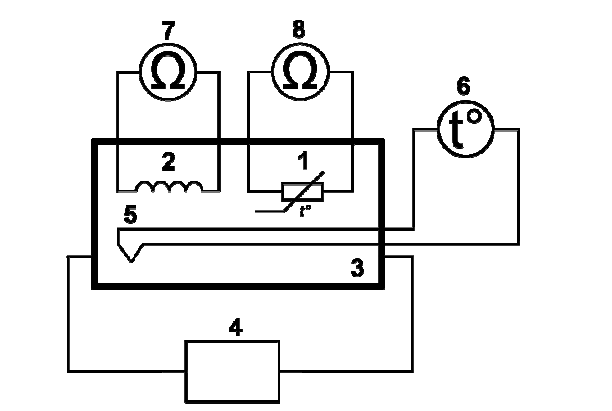
\includegraphics[width=10cm]{1}
				\vspace{2mm}
				\caption{Принципиальная схема лабораторной установки: 1 --- полупроводниковый терморезистор, 2 --- металлический терморезистор, 3 --- нагреватель, 4 --- блок питания HY3002, 5 --- термопара, 6 --- мультиметр DT9208 (термометр), 7, 8 --- мультиметры DT9205A (омметры)}
				\label{fig:setup}
			\end{minipage}
		\end{center}
	\end{figure}
	
	\section{Порядок выполнения работы.}
	\begin{enumerate}
		\item Проверена правильность собранной схемы: блок питания HY3002 подключён к гнёздам «Питание нагревателя $U = 10$--$15$ В», мультиметры DT9205A находятся в режиме омметра, кнопка включения и тумблер питания --- в положении «ВЫКЛ», регулятор напряжения выведен против часовой стрелки до упора.
		\newpage
		\item Измерено сопротивление полупроводникового и металлического терморезисторов при комнатной температуре.
		\item Включён источник питания, установлено напряжение нагревателя $10$ В и измерены зависимости $R_1(T)$ и $R_2(T)$ при нагревании от комнатной температуры до $70\,^\circ$C с шагом $2\,^\circ$C.
		\item Выключен источник питания и сняты зависимости $R_1(T)$ и $R_2(T)$ при остывании в интервале температур $68$--$30\,^\circ$C.
		\item Построены графики $R_1(T)$ и $R_2(T)$ для металлического и полупроводникового терморезисторов.
		\item Построен график $\ln R_1 = f(10^3/T)$ для полупроводникового терморезистора при нагревании и охлаждении, определена величина $B$ по тангенсу угла наклона прямой.
		\item Рассчитана величина $B$ по формуле \eqref{eq:B} для различных пар температур, результаты сравнены с п.~6.
		\item Определён ТКС металлического терморезистора по тангенсу угла наклона экспериментальной прямой $R_2(T)$, установлен материал терморезистора.
		\item Построена зависимость $\alpha = f(T)$ для полупроводникового терморезистора по формуле \eqref{eq:alpha}.
		\item По формуле \eqref{eq:dE} определена энергия активации проводимости $\Delta E$ полупроводникового терморезистора.
	\end{enumerate}
	
	\section{Ход выполнения работы.}
	
	\subsection{Таблицы с результатами прямых измерений.}
	В таблице~\ref{tab:data} приведены значения температуры и сопротивлений, полученные при нагревании (№~1--26), а затем при охлаждении (№~27--46) образцов.
	
	\begin{table}[H]
		\caption{Результаты измерений сопротивления при изменении температуры}
		\label{tab:data}
		\centering
		\small
		\begin{tabular}{|c|c|c|c||c|c|c|c|}
			\hline
			\multicolumn{4}{|c||}{Нагревание} & \multicolumn{4}{c|}{Охлаждение} \\
			\hline
			№ & $T$, $^\circ$C & $R_1$, кОм & $R_2$, кОм & № & $T$, $^\circ$C & $R_1$, кОм & $R_2$, кОм \\
			\hline
			1 & 20 & 4,80 & 0,393 & 27 & 68 & 1,49 & 0,465 \\
			2 & 22 & 4,70 & 0,397 & 28 & 66 & 1,52 & 0,458 \\
			3 & 24 & 4,51 & 0,401 & 29 & 64 & 1,55 & 0,456 \\
			4 & 26 & 4,36 & 0,393 & 30 & 62 & 1,61 & 0,456 \\
			5 & 28 & 4,21 & 0,379 & 31 & 60 & 1,67 & 0,450 \\
			6 & 30 & 3,91 & 0,410 & 32 & 58 & 1,77 & 0,445 \\
			7 & 32 & 3,75 & 0,409 & 33 & 56 & 1,84 & 0,446 \\
			8 & 34 & 3,56 & 0,417 & 34 & 54 & 1,94 & 0,444 \\
			9 & 36 & 3,45 & 0,421 & 35 & 52 & 2,03 & 0,440 \\
			10 & 38 & 3,22 & 0,425 & 36 & 50 & 2,09 & 0,438 \\
			11 & 40 & 3,04 & 0,430 & 37 & 48 & 2,23 & 0,434 \\
			12 & 42 & 2,89 & 0,434 & 38 & 46 & 2,35 & 0,432 \\
			13 & 44 & 2,79 & 0,439 & 39 & 44 & 2,45 & 0,429 \\
			14 & 46 & 2,61 & 0,445 & 40 & 42 & 2,59 & 0,426 \\
			15 & 48 & 2,50 & 0,444 & 41 & 40 & 2,71 & 0,424 \\
			16 & 50 & 2,40 & 0,445 & 42 & 38 & 2,88 & 0,421 \\
			17 & 52 & 2,26 & 0,442 & 43 & 36 & 3,02 & 0,420 \\
			18 & 54 & 2,14 & 0,447 & 44 & 34 & 3,19 & 0,417 \\
			19 & 56 & 2,06 & 0,452 & 45 & 32 & 3,35 & 0,413 \\
			20 & 58 & 1,94 & 0,459 & 46 & 30 & 3,54 & 0,410 \\
			21 & 60 & 1,85 & 0,462 &  & & &  \\
			22 & 62 & 1,78 & 0,464 &  & & &  \\
			23 & 64 & 1,70 & 0,467 &  & & &  \\
			24 & 66 & 1,64 & 0,467 &  & & &  \\
			25 & 68 & 1,57 & 0,468 &  & & &  \\
			26 & 70 & 1,49 & 0,470 &  & & &  \\
			\hline
		\end{tabular}
	\end{table}
	
	\subsection{Графики экспериментальных зависимостей.}
	
	\begin{figure}[H]
		\centering
		\begin{tikzpicture}
			\begin{axis}[
				width=0.94\textwidth,
				height=8cm,
				xlabel={$T$, $^\circ$C},
				ylabel={$R_1$, кОм},
				xmin=20, xmax=70,
				ymin=1.2, ymax=5.1,
				xtick={20,25,30,35,40,45,50,55,60,65,70},
				grid=major,
				tick label style={font=\small},
				label style={font=\normalsize},
				legend pos=north east,
				legend style={font=\small},
				]
				\addplot[only marks,mark=*,mark size=1.8pt,blue] coordinates {
					(20,4.80) (22,4.70) (24,4.51) (26,4.36) (28,4.21)
					(30,3.91) (32,3.75) (34,3.56) (36,3.45) (38,3.22)
					(40,3.04) (42,2.89) (44,2.79) (46,2.61) (48,2.50)
					(50,2.40) (52,2.26) (54,2.14) (56,2.06) (58,1.94)
					(60,1.85) (62,1.78) (64,1.70) (66,1.64) (68,1.57) (70,1.49)
				};
				\addlegendentry{Нагревание}
				\addplot[only marks,mark=square*,mark size=1.6pt,red!75!black] coordinates {
					(68,1.49) (66,1.52) (64,1.55) (62,1.61) (60,1.67)
					(58,1.77) (56,1.84) (54,1.94) (52,2.03) (50,2.09)
					(48,2.23) (46,2.35) (44,2.45) (42,2.59) (40,2.71)
					(38,2.88) (36,3.02) (34,3.19) (32,3.35) (30,3.54)
				};
				\addlegendentry{Охлаждение}
			\end{axis}
		\end{tikzpicture}
		\caption{Зависимость сопротивления $R_1$ полупроводникового терморезистора от температуры}
		\label{fig:r1}
	\end{figure}
	
	\begin{figure}[H]
		\centering
		\begin{tikzpicture}
			\begin{axis}[
				width=0.94\textwidth,
				height=8cm,
				xlabel={$T$, $^\circ$C},
				ylabel={$R_2$, кОм},
				xmin=20, xmax=70,
				ymin=0.38, ymax=0.48,
				xtick={20,25,30,35,40,45,50,55,60,65,70},
				ytick={0.38,0.40,0.42,0.44,0.46,0.48},
				grid=major,
				tick label style={font=\small},
				label style={font=\normalsize},
				legend pos=south east,
				legend style={font=\small},
				]
				\addplot[only marks,mark=*,mark size=1.8pt,blue] coordinates {
					(20,0.393) (22,0.397) (24,0.401) (26,0.393) (28,0.379)
					(30,0.410) (32,0.409) (34,0.417) (36,0.421) (38,0.425)
					(40,0.430) (42,0.434) (44,0.439) (46,0.445) (48,0.444)
					(50,0.445) (52,0.442) (54,0.447) (56,0.452) (58,0.459)
					(60,0.462) (62,0.464) (64,0.467) (66,0.467) (68,0.468) (70,0.470)
				};
				\addlegendentry{Нагревание}
				\addplot[only marks,mark=square*,mark size=1.6pt,red!75!black] coordinates {
					(68,0.465) (66,0.458) (64,0.456) (62,0.456) (60,0.450)
					(58,0.445) (56,0.446) (54,0.444) (52,0.440) (50,0.438)
					(48,0.434) (46,0.432) (44,0.429) (42,0.426) (40,0.424)
					(38,0.421) (36,0.420) (34,0.417) (32,0.413) (30,0.410)
				};
				\addlegendentry{Охлаждение}
				\addplot[black, thick, domain=20:70, samples=2] {0.3607 + 0.0015872*x};
				\addlegendentry{Линейная аппроксимация}
			\end{axis}
		\end{tikzpicture}
		\caption{Зависимость сопротивления $R_2$ металлического терморезистора от температуры}
		\label{fig:r2}
	\end{figure}
	
	\begin{figure}[H]
		\centering
		\begin{tikzpicture}
			\begin{axis}[
				width=0.94\textwidth,
				height=8cm,
				xlabel={$10^3/T$, К$^{-1}$},
				ylabel={$\ln R_1$ ($R_1$ в кОм)},
				xmin=2.9, xmax=3.43,
				ymin=0.3, ymax=1.7,
				grid=major,
				tick label style={font=\small},
				label style={font=\normalsize},
				legend pos=north west,
				legend style={font=\small},
				]
				\addplot[only marks,mark=*,mark size=1.8pt,blue] table[row sep=\\, x expr=1000/(\thisrow{T}+273.15), y expr=ln(\thisrow{R})] {
					T R \\
					20 4.80 \\ 22 4.70 \\ 24 4.51 \\ 26 4.36 \\ 28 4.21 \\ 30 3.91 \\ 32 3.75 \\ 34 3.56 \\ 36 3.45 \\ 38 3.22 \\
					40 3.04 \\ 42 2.89 \\ 44 2.79 \\ 46 2.61 \\ 48 2.50 \\ 50 2.40 \\ 52 2.26 \\ 54 2.14 \\ 56 2.06 \\ 58 1.94 \\
					60 1.85 \\ 62 1.78 \\ 64 1.70 \\ 66 1.64 \\ 68 1.57 \\ 70 1.49 \\
				};
				\addlegendentry{Нагревание}
				\addplot[only marks,mark=square*,mark size=1.6pt,red!75!black] table[row sep=\\, x expr=1000/(\thisrow{T}+273.15), y expr=ln(\thisrow{R})] {
					T R \\
					68 1.49 \\ 66 1.52 \\ 64 1.55 \\ 62 1.61 \\ 60 1.67 \\ 58 1.77 \\ 56 1.84 \\ 54 1.94 \\ 52 2.03 \\ 50 2.09 \\
					48 2.23 \\ 46 2.35 \\ 44 2.45 \\ 42 2.59 \\ 40 2.71 \\ 38 2.88 \\ 36 3.02 \\ 34 3.19 \\ 32 3.35 \\ 30 3.54 \\
				};
				\addlegendentry{Охлаждение}
				\addplot[blue, thick, domain=2.91:3.41, samples=2] {-6.728 + 2.4516*x};
				\addlegendentry{Аппроксимация (нагревание)}
				\addplot[red!75!black, thick, dashed, domain=2.91:3.41, samples=2] {-6.810 + 2.4458*x};
				\addlegendentry{Аппроксимация (охлаждение)}
			\end{axis}
		\end{tikzpicture}
		\caption{Зависимость $\ln R_1 = f(10^3/T)$ при нагревании и охлаждении}
		\label{fig:lnR}
	\end{figure}
	
	\subsection{Расчёт постоянной $B$ и энергии активации.}
	Линейная аппроксимация методом наименьших квадратов (рис.~\ref{fig:lnR}) даёт: при нагревании $\operatorname{tg}\varphi_{\text{н}} = 2,452$ ($R^2 = 0,9969$), при охлаждении $\operatorname{tg}\varphi_{\text{о}} = 2,446$ ($R^2 = 0,9978$). Отсюда
	\[
	B_{\text{н}} = 10^3 \cdot 2,452 \approx 2452 \text{ К}, \qquad B_{\text{о}} = 10^3 \cdot 2,446 \approx 2446 \text{ К},
	\]
	\[
	B = \frac{B_{\text{н}} + B_{\text{о}}}{2} \approx 2449 \text{ К}.
	\]
	Свободный член прямых даёт $R_0 \approx 1,2$ Ом (нагревание) и $R_0 \approx 1,1$ Ом (охлаждение).
	
	Для сравнения $B$ рассчитана по формуле \eqref{eq:B} по данным ветви нагревания для нескольких пар температур (табл.~\ref{tab:B}). Например, для $T_1 = 293{,}15$ К ($20\,^\circ$C, $R = 4{,}80$ кОм) и $T_2 = 343{,}15$ К ($70\,^\circ$C, $R = 1{,}49$ кОм):
	\[
	B = \frac{293{,}15 \cdot 343{,}15}{343{,}15 - 293{,}15} \ln \frac{4{,}80}{1{,}49} \approx 2354 \text{ К}.
	\]
	
	\begin{table}[H]
		\caption{Постоянная $B$, рассчитанная по формуле \eqref{eq:B} для разных пар температур}
		\label{tab:B}
		\centering
		\begin{tabular}{|c|c|c|c|c|}
			\hline
			$T_1$, $^\circ$C & $T_2$, $^\circ$C & $R(T_1)$, кОм & $R(T_2)$, кОм & $B$, К \\
			\hline
			20 & 70 & 4.80 & 1.49 & 2 354 \\ \hline
			20 & 60 & 4.80 & 1.85 & 2 328 \\ \hline
			20 & 50 & 4.80 & 2.40 & 2 189 \\ \hline
			30 & 70 & 3.91 & 1.49 & 2 509 \\ \hline
			30 & 60 & 3.91 & 1.85 & 2 519 \\ \hline
			40 & 70 & 3.04 & 1.49 & 2 554 \\ \hline
		\end{tabular}
	\end{table}
	
	Среднее по парам $B_{\text{ср}} \approx 2409$ К, разброс от 2189 до 2554 К.
	
	Энергия активации проводимости по формуле \eqref{eq:dE}:
	\[
	\Delta E = kB = 8{,}617 \cdot 10^{-5} \cdot 2449 \approx 0,211 \text{ эВ},
	\]
	что соответствует ширине запрещённой зоны $E_g = 2\Delta E \approx 0,422$ эВ.
	
	\subsection{Расчёт ТКС.}
	Для полупроводникового терморезистора ТКС рассчитан по формуле \eqref{eq:alpha} при $B = 2449$ К (табл.~\ref{tab:alpha}), например при $T = 293{,}15$ К:
	\[
	\alpha = -\frac{B}{T^2} = -\frac{2449}{293{,}15^2} \approx --2,85 \cdot 10^{-2} \text{ К}^{-1}.
	\]
	
	\begin{table}[H]
		\caption{Температурная зависимость ТКС полупроводникового терморезистора}
		\label{tab:alpha}
		\centering
		\begin{tabular}{|c|c|c|}
			\hline
			$T$, $^\circ$C & $T$, К & $\alpha$, $10^{-2}$ К$^{-1}$ \\
			\hline
			20 & 293 & -2,85 \\ \hline
			30 & 303 & -2,66 \\ \hline
			40 & 313 & -2,50 \\ \hline
			50 & 323 & -2,34 \\ \hline
			60 & 333 & -2,21 \\ \hline
			70 & 343 & -2,08 \\ \hline
		\end{tabular}
	\end{table}
	
	Для металлического терморезистора линейная аппроксимация по всем точкам (рис.~\ref{fig:r2}) даёт $R_2(T) = 0.3607 + 0.0015872\,T$ (кОм, $T$ в $^\circ$C). Наклон $\Delta R_2/\Delta T = 1,59 \cdot 10^{-3}$ кОм/К, сопротивление при $20\,^\circ$C $R_{20} = 0,392$ кОм. По формуле \eqref{eq:alphaM}:
	\[
	\alpha_2 = \frac{1}{R_{20}}\frac{\Delta R_2}{\Delta T} = \frac{1,59 \cdot 10^{-3}}{0,392} \approx +4,04 \cdot 10^{-3} \text{ К}^{-1}.
	\]
	Полученное значение близко к табличному ТКС меди ($\approx 4{,}3 \cdot 10^{-3}$ К$^{-1}$, отличие около 6\%), что подтверждает, что металлический терморезистор изготовлен из меди.
	
	\section{Оценка ошибок измерений и вычислений.}
	Основные источники погрешности: дискретность отсчёта температуры ($\pm 1\,^\circ$C), погрешность омметра DT9205A и тепловая инерция установки.
	
	Относительная погрешность определения $B$ по разным парам точек (табл.~\ref{tab:B}):
	\[
	\delta_B = \frac{B_{\max} - B_{\min}}{B_{\text{ср}}} \cdot 100\% \approx 15\%.
	\]
	Значения $B$ по двум ветвям (нагревание и охлаждение) совпадают в пределах $0{,}2\%$: $B_{\text{н}} = 2452$ К, $B_{\text{о}} = 2446$ К.
	
	Для металлического терморезистора разброс точек $R_2(T)$ заметен при $T < 30\,^\circ$C (например, $R_2(28\,^\circ\text{C}) = 0{,}379$ кОм ниже соседних значений), так как изменение $R_2$ составляет всего около $20\%$ на всём интервале и сопоставимо с погрешностью омметра.
	
	\section{Выводы.}
	\subsection*{Анализ экспериментальных данных.}
	Исследована зависимость сопротивлений двух образцов от температуры. Сопротивление $R_1$ с ростом температуры уменьшается (полупроводниковый терморезистор, $\alpha < 0$), $R_2$ в целом увеличивается (металлический терморезистор, $\alpha > 0$). В координатах $\ln R_1 = f(10^3/T)$ данные ложатся на прямые ($R^2 > 0{,}99$), что подтверждает закон \eqref{eq:R}. Получено $B \approx 2449$ К, $\alpha_1 \approx --2,85 \cdot 10^{-2}$ К$^{-1}$ при $20\,^\circ$C, $\Delta E \approx 0,211$ эВ; для металлического терморезистора $\alpha_2 \approx 4,04 \cdot 10^{-3}$ К$^{-1}$, материал --- медь.
	
	\subsection*{Сопоставление с теорией.}
	Рост $R_1$ при охлаждении и его падение при нагревании соответствуют экспоненциальному росту числа носителей заряда с температурой, а рост $R_2$ --- усилению рассеяния электронов на фононах. Постоянная $B$ не является строго постоянной: по разным парам температур она меняется от 2189 до 2554 К, что соответствует замечанию методических указаний о зависимости $B$ от температуры для реальных терморезисторов. $|\alpha_1|$ уменьшается с ростом температуры как $1/T^2$ (табл.~\ref{tab:alpha}).
	
	\newpage
	\subsection*{Критические замечания.}
	Ветви нагревания и охлаждения $R_1(T)$ не совпадают: при одной и той же температуре сопротивление при охлаждении меньше (например, при $40\,^\circ$C $3{,}04$ кОм против $2{,}71$ кОм). Это объясняется тепловой инерцией: термопара и образец прогреваются и остывают с разной скоростью, поэтому показание термометра отстаёт от реальной температуры образца. Опыт ограничен интервалом до $70\,^\circ$C, измерения при охлаждении начаты с $68\,^\circ$C и закончены на $30\,^\circ$C, поэтому для повышения точности нужны более медленный нагрев и выдержка перед отсчётом. Цель достигнута.
	
	\newpage
	\section*{Список литературы}
	\addcontentsline{toc}{section}{Список литературы}
	
	\begin{enumerate}
		\item Изучение терморезистора~: метод. указания / сост.~Н.~А.~Рудь, А.~Н.~Сергеев ; Яросл. гос. ун-т им.~П.~Г.~Демидова.~-- Ярославль~: ЯрГУ, 2011.~-- 60~с.
		\item Сивухин, Д.~В. Курс общей физики~: в 5~т. Т.~5. Атомная и ядерная физика~: учебное пособие / Д.~В.~Сивухин.~-- 3-е изд., стер.~-- Москва~: ФИЗМАТЛИТ, 2002.~-- 784~с.~-- ISBN 5-9221-0230-4.
	\end{enumerate}
	
\end{document}